\title{\emph{Walking In Wollaton}\\
       Report for G54MRT Coursework 1
       }
\author{}
\date{}
\documentclass[12pt, a4paper]{article}

\usepackage{graphicx}
\graphicspath{{Images/}}

\begin{document}
\maketitle

\section{Design}
\subsection{Summary}
The objective of the game is to encourage users to explore all areas of Wollaton Hall, and by extension Wollaton Park.
The game will aim to take a user on a "guided tour" of the grounds by providing the user with a series of "collectables" relating to exhibits in the museum that makes up Wollaton Hall, and some of the surrounding landmarks such as Wollaton Park Lake.
These areas will be defined based on the map in Figure \ref{fig:wollatonmap}.

\begin{figure}[ht]
  \centering
  \caption{A map of the Wollaton Park grounds, taken from www.wollatonhall.org.uk/visit}
  \includegraphics[width=\textwidth]{wollaton-park-map.png}
  \label{fig:wollatonmap}
\end{figure}

The main consideration that should be taken here is that users do not stray onto either the deer sanctuary in the northwest corner or the golf course that makes up much of the southeast of the park.
The game will be prototyped using the WanderAnywhere platform, mainly because it will be more of the form of a "walking simulator" a la \textit{Dear Esther}.

\subsection{Ideation Cards}
I will take 3 ideation cards from each category and in the following section outline my responses to them.

\subsubsection{Opportunities}
\begin{itemize}
  \item Scavenger Hunt - Players travel between locations to find clues or treasures\\
        The whole objective of the game is that players move between locations and "collect" treasures in the form of experiences.
  \item Unusual Locations - Players get to visit places they otherwise would not\\
        Again, the nature of the game is such that it will hopefully encourage people to explore a greater area of the Park grounds than they otherwise would, and potentially even parts of the museums on said grounds that they would ordinarily ignore.
  \item Exergaming - The game requires acts of endurance, strength, or dexterity\\
        The gamification aspect of the experience means that a user could be scored on how long it takes them to "collect" a set number of objectives - this may mean visiting 8 unique areas and the fastest time wins.
        In a more realised version of the game it may be preferable that the game become social, and that a group of users select the locations to explore and race one another.
\end{itemize}

\subsubsection{Questions}
\begin{itemize}
  \item Duration - How long is a game session? Should it be shorter or longer?\\
        The duration of the game is the scoring system in a sense, so this aspect will refer to the number of objectives to be explored before a session is considered finished.
        Ideally the game will take no more than a couple of hours to finish at a leisurely pace, although speedrunners exist for all forms of video game.
  \item Experience Flow - How do players journey through the game?\\
        The users will journey from point to point around the park, likely staying to the west of the house given that the east is made up mostly of the golf course, a play area, and a walled garden to which the public has no access.
  \item Indoor / Outdoor - Can the game be played in both? Should it? What would change?\\
        By its nature the game will be played in both, although given a larger museum it could be adapted to be entirely indoors.
        I feel that the dual nature of the game will ultimately make it more enjoyable - with potential for different game modes including an entirely indoors version for less weather-conducive days.
\end{itemize}

\subsubsection{Challenges}
\begin{itemize}
  \item Long Distances - How are players engaged while between game locations?\\
        This is in my view the greatest challenge the game will face, and will depend greatly on the chosen path between objectives.
        Ideally the game will provide information about the history of the grounds or information on local wildlife in between locations, however this may be redundant if some of the objectives relate to those topics.
  \item Phone Zombies - Will players be staring at their screens most of the time?\\
        Again this is a matter of the design of the game at the "in-between" phase, as at each point the game should be set up such that it encourages the user to not look at their screens until it is time to go to another location.
  \item Unstable Connectivity - How does the game continue without a data connection?\\
        The full version of the game should contain locally all of the required information for the game to continue sans data.
\end{itemize}

\subsection{Concept Sketch}

Figure \ref{fig:concept} shows the concept poster for the game, including all ideation cards used.
The game is centered at the Hall, and every time the player goes to a location and back they are given a new randomly selected location to go to.
They are timed while en route between the Hall and the location given, but not at the locations themselves (however they will only have 10 minutes maximum at each before they are warned to get back to the Hall for the next location).

\begin{figure}[ht]
\centering
  \caption{The concept poster for the game}
  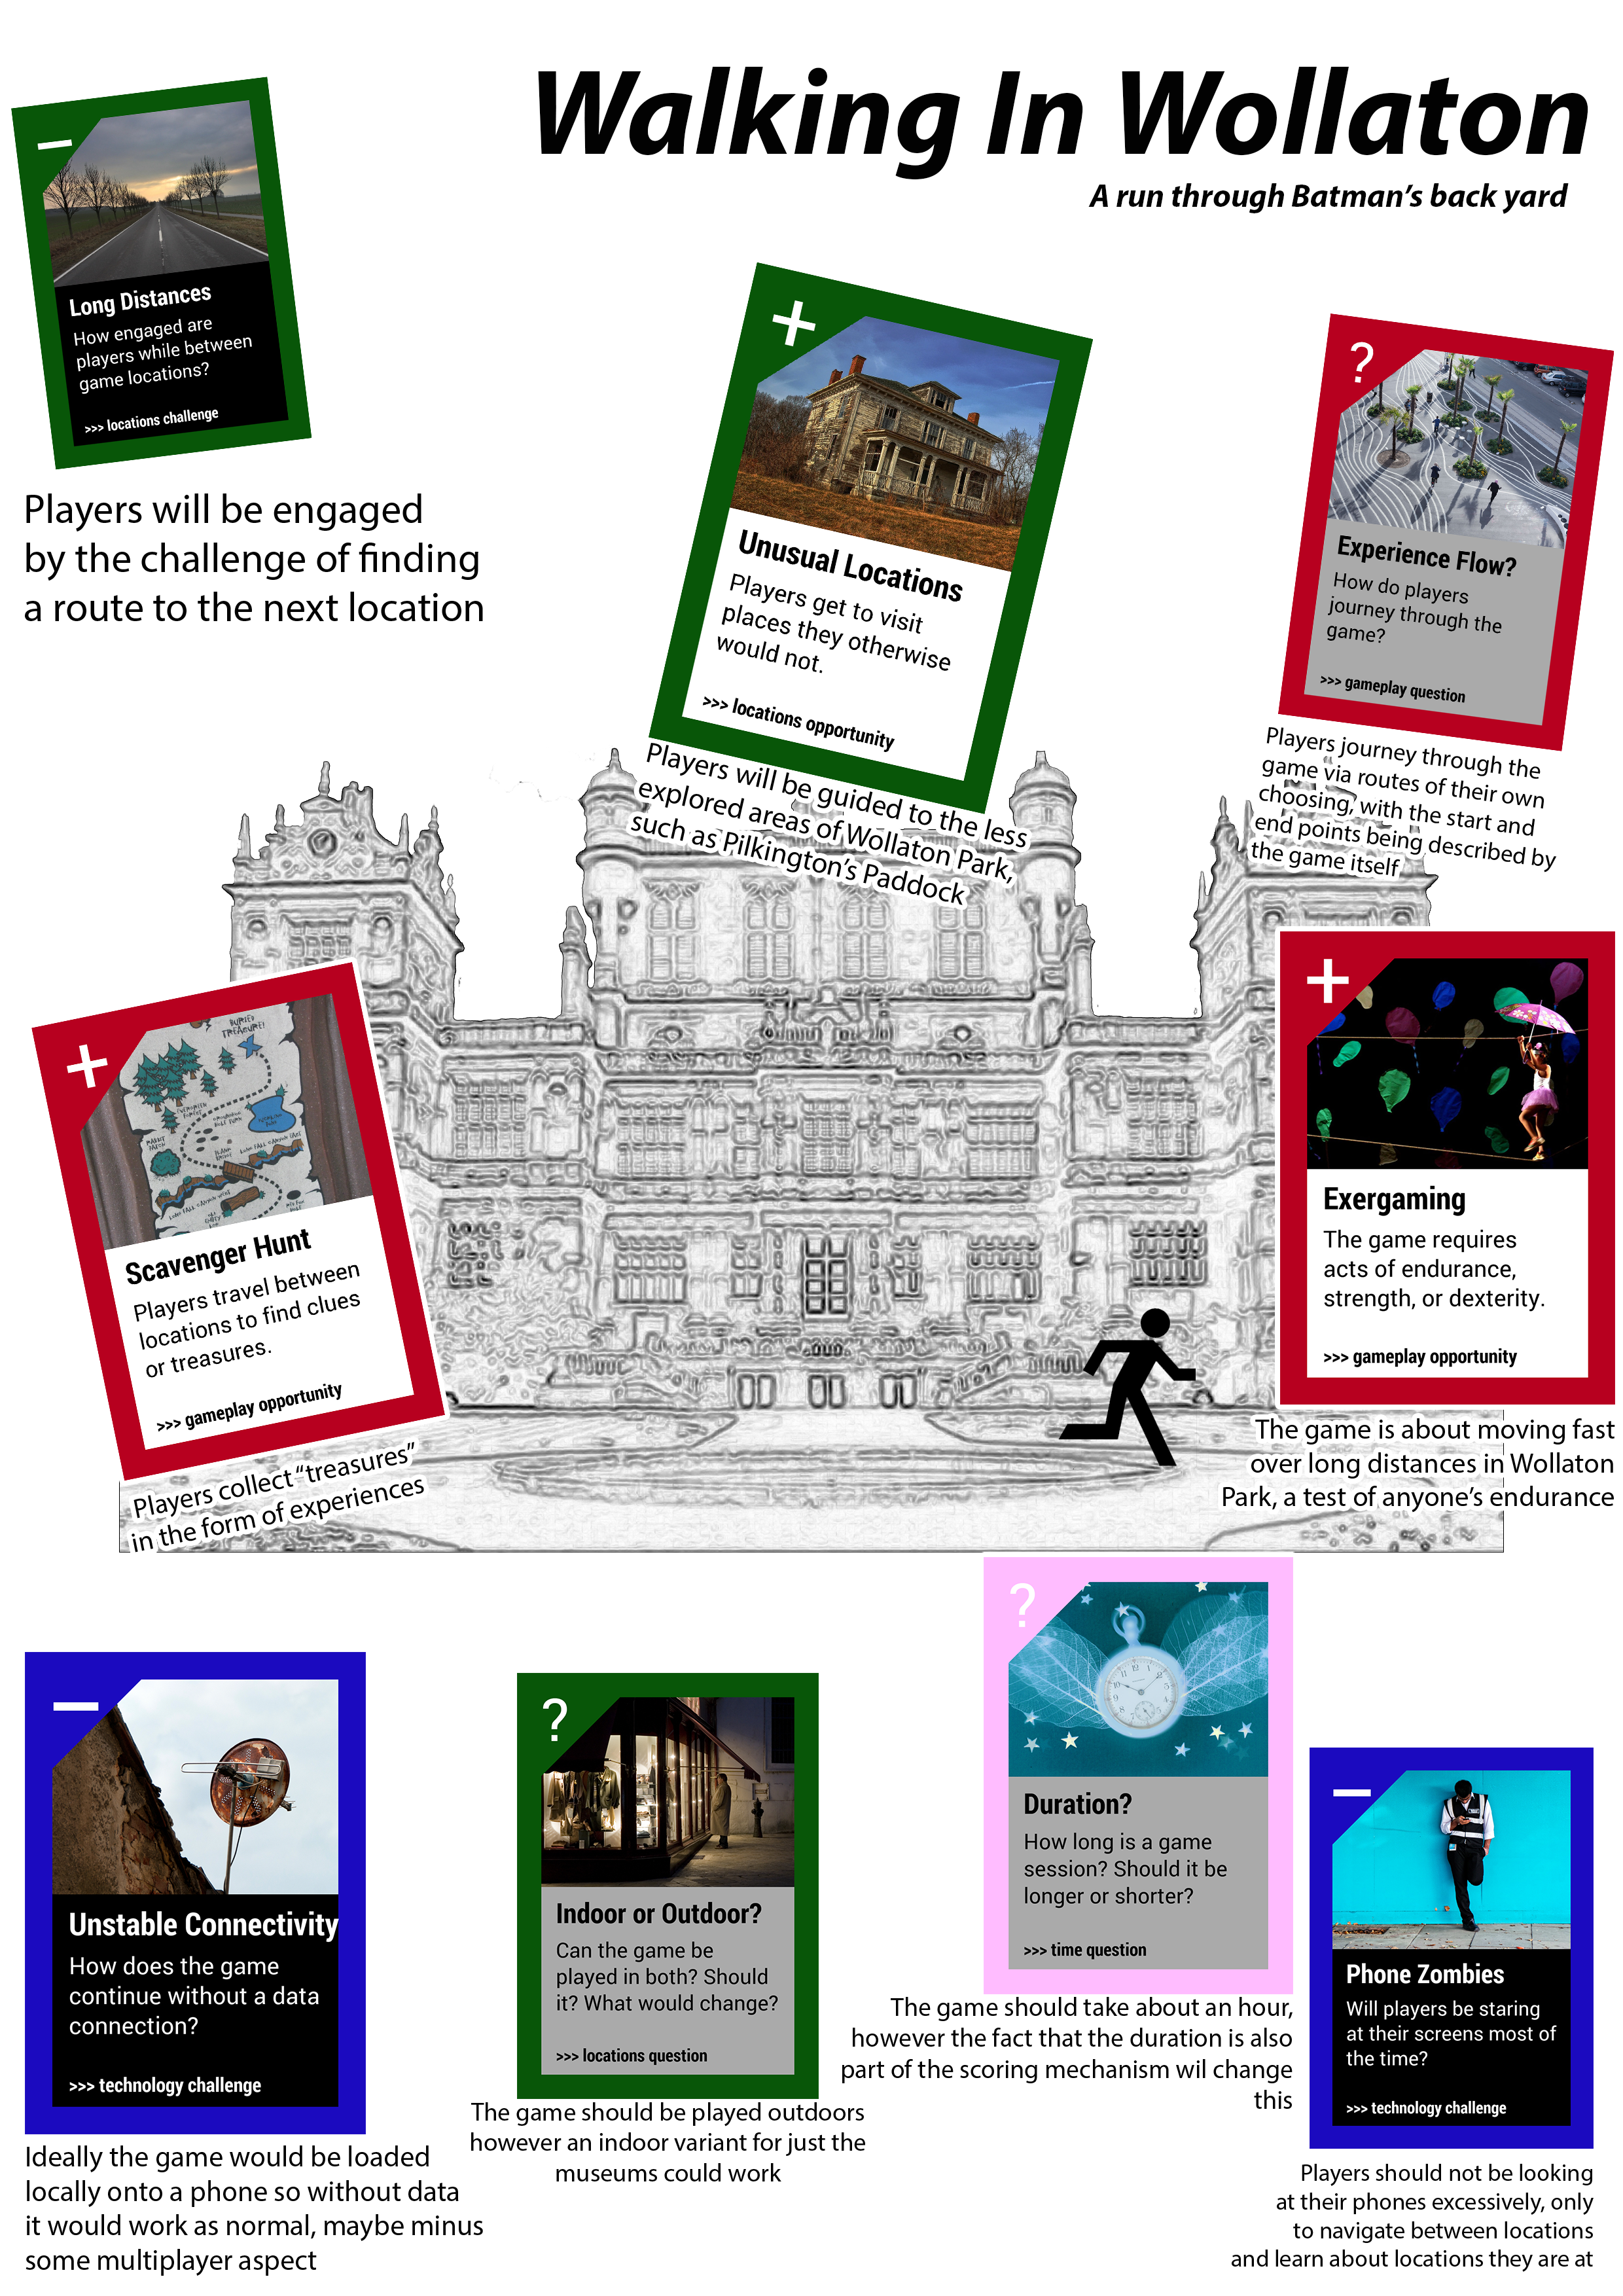
\includegraphics[width=0.7\textwidth]{conceptposter.png}
  \label{fig:concept}
\end{figure}

\section{Prototype}

I prototyped the application using \textit{Wander Anywhere}, an online locative media authoring service.
The prototype is somewhat basic, essentially only plotting a single route through the park, however I believe it works well as a proof of concept.
If the user is generally within the grounds of the park, the application invites them to go to the front drive of the Hall, where the trail begins.
It then gets them to go to, in order:
\begin{enumerate}
  \item Beeston Lodge
  \item Wollaton Lake
  \item Thompson's Wood
  \item Pilkington's Paddock
  \item Camellia House
  \item The Industrial Museum
  \item The Museum of Natural History
\end{enumerate}

It does not time or fully direct the user (only giving broad location-to-location compass directions), however it does provide them with some information about each new location they discover.

The annotated photostory can be seen in Figure \ref{fig:photostory}.

\begin{figure}[ht]
\centering
  \caption{Annotated photostory of the prototype.}
  \includegraphics[height=18cm]{photostory.png}
  \label{fig:photostory}
\end{figure}

\section{Testing}
\subsection{Testing Process}
The testing process is somewhat simple: go to Wollaton Park and go along the route, checking to ensure that directions are valid and that locations are not overlapped or inaccessible.
Screenshots can be seen in Figure \ref{fig:testingProof}.

\begin{figure}[ht]
\centering
  \caption{Screenshots from each major location in the game.}
  \includegraphics[width=0.5\textwidth]{testingProof.png}
  \label{fig:testingProof}
\end{figure}

\subsection{Issues Revealed}
\begin{itemize}
  \item There is some overlap between the Thompson's Wood and Lake sections of the experience - this could probably be solved by implementing a point marker to aim for once the user is in the broad area.
  \item The Beeston Lodge target, as the crow flies, is directly across the golf course from Wollaton Hall.
A user may, in the pursuit of the lowest time, cross this course, which is illegal.
  \item Going from location to location there is a lack of provided entertainment from the game - possibly fixable with more locations or some general AR games/Easter Eggs (e.g. take a picture of a deer).
  \item The area in Thompson's Wood that the prototype has the user go to is not the area in which dens are built (per the photostory) - this has been changed to more accurately represent the area.
        This update also makes the route for the user more linear and interesting.
  \item There is some amount of "returning to previous locations" involved with the route, in particular if the user takes the proper route to Beeston Lodge they pass close enough to the lake that they nearly unlock that location.
        Short of moving the bounds of the lake section to within the lake there is no real way around this unfortunately.
\end{itemize}


\section{Critical Reflection}
Overall this prototype is a fair reflection of one path of the game.
Wander Anywhere's non-directionality (i.e. the fact that you cannot trigger one location becoming available by going to another) means that implementing the "return to the Hall" functionality is not possible, however I am happy that the routes the game encourages you to take are valid.
The only exception to this is the Beeston Lodge route: if a player is really going for the lowest time possible they are likely to try and cut through the golf course, which is illegal given that the course is private.
From this it may be worth either removing the "return to base" feature or otherwise spoofing a route using the compass direction indicator to "trick" the user into going around the course rather than through it.

\subsection{Specific Concepts}
This is a piece of purely locative media; it relies entirely on the users' location to provide it with the information it needs to give the user the best possible version of the intended experience.
In a final version of the application it would load the section of the map containing Wollaton Park only and keep it stored for the duration of the game, in order to not rely on the cellular signal within the Park - downloading and installing content is obviously very inconvenient for a user but the game crashing because of a dropped connection while a user is trying to get from Beeston Lodge to Pilkington's Paddock as quickly as possible will ruin the entire experience for them.
I used the concept of specific locations for each individual target - I feel that the game subverts these locations somewhat given that Wollaton Park is a fairly quiet place most of the time, and the game is deliberately fast-paced, giving an interesting contrast to the general feel of the Park as a whole.
In terms of the concept of routes the game does not provide users with specific routes, rather locations to which the users must navigate themselves.
Again, the Beeston Lodge issue makes this something of a problem, as I feel that giving a user a route makes the game less "orienteering" and more "cross-country running", which is not the objective.
\par
The triggers are designed considering the temporal aspect; in particular the "base" location of Wollaton Hall changes its state depending on where the user has gone to since leaving it previously.
I aimed to avoid an eyes-down experience by providing a minimal amount of data to the user while they are travelling between locations - only a compass in the eventual game, but the Wander Anywhere map is a similar concept so I am happy that it is not likely to be a phone zombie situation.

\end{document}
